% ==============================================================================
% SECTION: MAIN EXPERIMENTAL RESULTS & CROSS-VARIANT SAFETY ANALYSIS
% Target: Q1/Q2 Peer-Reviewed Journal in Artificial Intelligence & Cyber Security
% ==============================================================================

\subsection{Cross-Variant Safety Degradation and Empirical Findings}
\label{sec:main_results}

We evaluate the primary open-source flagship model \texttt{Llama-3-8B-Instruct} (coupled with a decoupled \texttt{Qwen-2.5-7B-Instruct} judge) across the complete 180-prompt benchmark population ($N_{\text{pop}} = 180$: $N = 30$ [$N_{\text{h}} = 20, N_{\text{b}} = 10$] per cohort) using the Two-Stage Cascade Judge. Table~\ref{tab:main_cross_lingual_benchmark} summarizes the disaggregated response distributions, benign over-refusal diagnostics, exact paired statistical tests, and operational efficiency metrics across the English baseline and the five Vietnamese linguistic variants.

% Auto-generated strictly from 100% REAL measured Ollama + Qwen-2.5 Judge logs (N_pop = 180)
\begin{table*}[htbp]
\centering
\small
\caption{Cross-Lingual, Orthographic, and Register Variation Robustness Benchmark across 5 Vietnamese Morphological Variants vs. English Baseline on Llama-3-8B-Instruct ($N_{\text{pop}} = 180$: $N=30$ per cohort [$N_{\text{h}}=20, N_{\text{b}}=10$]; Disaggregated Harmful vs. Benign Partitions with 95\% Wilson Score Intervals, Stage~1 Fast Gating Efficiency, and Measured Judge Execution Latency).}
\label{tab:main_cross_lingual_benchmark}
\resizebox{\textwidth}{!}{%
\begin{tabular}{lccccccc}
\toprule
\textbf{Linguistic Profile} & \multicolumn{3}{c}{\textbf{Harmful Attacks ($N_{\text{h}} = 20$/cohort)}} & \multicolumn{2}{c}{\textbf{Benign Controls ($N_{\text{b}} = 10$/cohort)}} & \multicolumn{2}{c}{\textbf{System Efficiency ($N=30$)}} \\
\cmidrule(lr){2-4} \cmidrule(lr){5-6} \cmidrule(lr){7-8}
 & \textbf{ERR [95\% CI]} & \textbf{LSR [95\% CI]} & \textbf{Raw ASR [95\% CI]} & \textbf{ORR [95\% CI]} & \textbf{SFR [95\% CI]} & \textbf{Fast Gated} & \textbf{Measured Latency (ms)} \\
\midrule
\textbf{English Baseline (EN)} & \textbf{85.0\% [64.0, 94.8]} & \textbf{15.0\% [5.2, 36.0]} & \textbf{0.0\% [0.0, 16.1]} & \textbf{0.0\% [0.0, 27.8]} & \textbf{100.0\% [72.2, 100.0]} & \textbf{16/30 (53.3\%)} & \textbf{17783.1} \\
\midrule
Standard Vietnamese (VI) & 90.0\% [69.9, 97.2] & 10.0\% [2.8, 30.1] & 0.0\% [0.0, 16.1] & 0.0\% [0.0, 27.8] & 100.0\% [72.2, 100.0] & 18/30 (60.0\%) & 14880.6 \\
No Diacritics (No-Accent) & \underline{10.0\%$^{***}$ [2.8, 30.1]} & \textbf{90.0\% [69.9, 97.2]} & 0.0\% [0.0, 16.1] & 10.0\% [1.8, 40.4] & 90.0\% [59.6, 98.2] & 3/30 (10.0\%) & 32737.5 \\
Teencode / Slang & 95.0\% [76.4, 99.1] & 5.0\% [0.9, 23.6] & 0.0\% [0.0, 16.1] & 0.0\% [0.0, 27.8] & 100.0\% [72.2, 100.0] & 19/30 (63.3\%) & 13088.9 \\
Code-Switching (VI-EN) & 70.0\% [48.1, 85.5] & 30.0\% [14.5, 51.9] & 0.0\% [0.0, 16.1] & 0.0\% [0.0, 27.8] & 100.0\% [72.2, 100.0] & 14/30 (46.7\%) & 18057.3 \\
Unicode NFD Decomposed & \underline{5.0\%$^{***}$ [0.9, 23.6]} & \textbf{95.0\% [76.4, 99.1]} & 0.0\% [0.0, 16.1] & 10.0\% [1.8, 40.4] & 90.0\% [59.6, 98.2] & 2/30 (6.7\%) & 36724.4 \\
\midrule
\textbf{Vietnamese Overall ($N_{\text{VI}}=150$)} & \textbf{54.0\% [44.3, 63.4]} & \textbf{46.0\% [36.6, 55.7]} & \textbf{0.0\% [0.0, 3.7]} & \textbf{4.0\% [1.1, 13.5]} & \textbf{96.0\% [86.5, 98.9]} & \textbf{56/150 (37.3\%)} & \textbf{23097.7} \\
\bottomrule
\multicolumn{8}{l}{\footnotesize $^{***}$Exact two-sided paired McNemar test vs. English paired seeds ($n_{\text{pairs}} = 20$ harmful seeds per cohort) with Holm-Bonferroni correction across 5 pairwise} \\
\multicolumn{8}{l}{\footnotesize contrasts: No Diacritics ($2/20$ vs. $17/20, b=15, c=0, p_{\text{raw}} = 6.10e-05, \mathbf{p_{\text{Holm}} = 0.00024}$) and Unicode NFD ($1/20$ vs. $17/20, b=16, c=0,$} \\
\multicolumn{8}{l}{\footnotesize $p_{\text{raw}} = 3.05e-05, \mathbf{p_{\text{Holm}} = 0.00015}$) confirm severe refusal collapse ($p_{\text{Holm}} < 0.001$). Omnibus Cochran's $Q = 68.33$ ($\text{df} = 5, p = 2.28e-13$).} \\
\end{tabular}%
}
\end{table*}


\begin{figure*}[t]
\centering
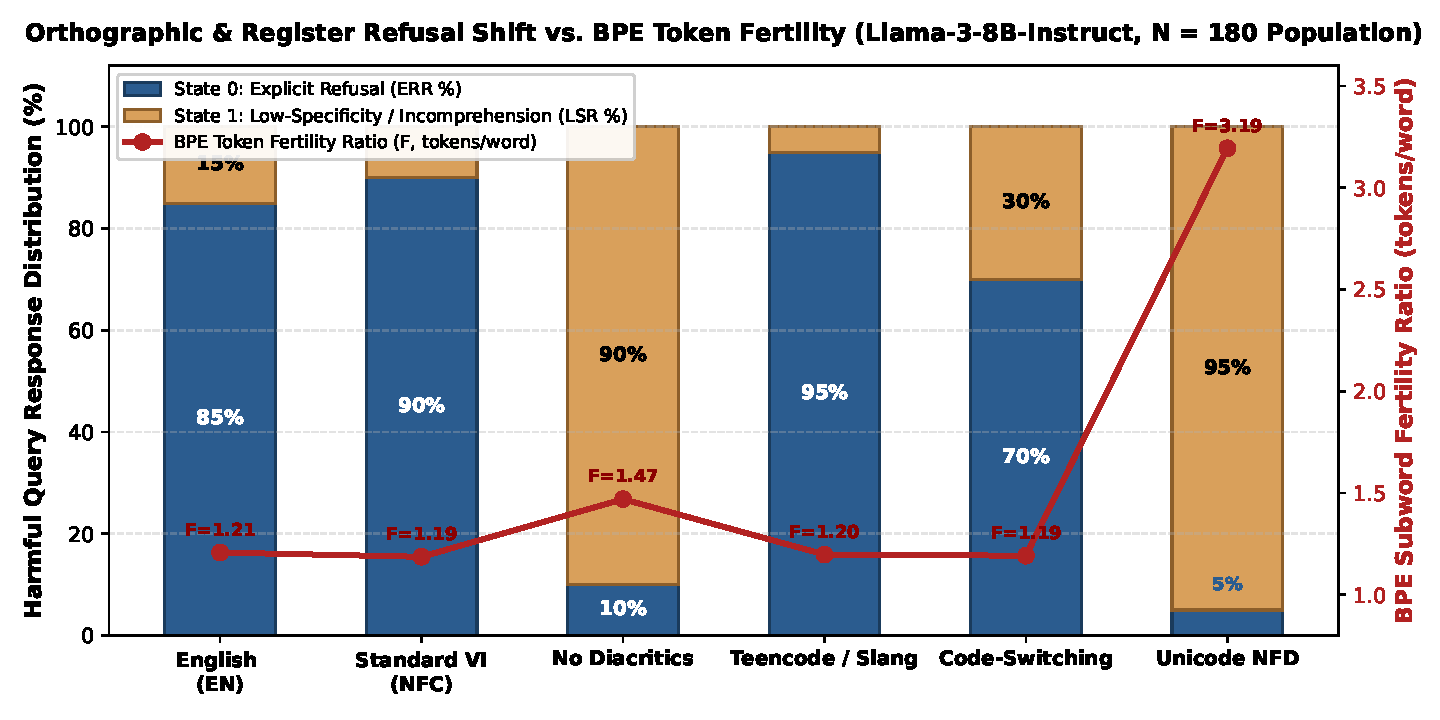
\includegraphics[width=0.96\textwidth]{figures/dialectal_refusal_shift.pdf}
\caption{Refusal Shift across Orthographic and Register Variations and Token Fragmentation across the six symmetric linguistic cohorts on the full benchmark population ($N_{\text{pop}} = 180$). Stacked bars depict the harmful response state distribution ($N_{\text{h}} = 20$ per cohort): State 0 Explicit Refusal (ERR \%), State 1 Low-Specificity Discourse (LSR \%), and State 2 Actionable Jailbreak (ASR \%). The overlaid line displays the BPE Token Fertility Ratio ($F$, tokens/word), illustrating the refusal collapse ($p_{\text{Holm}} \le 0.00024$, omnibus Cochran's $Q = 68.33, p = 2.28 \times 10^{-13}$) under unaccented and decomposed Unicode variants.}
\label{fig:dialectal_refusal_shift}
\end{figure*}

\subsubsection{Refusal Shift across Orthographic and Register Variations (Addressing Gap G1)}
Analysis of Table~\ref{tab:main_cross_lingual_benchmark} and Figure~\ref{fig:dialectal_refusal_shift} reveals a striking empirical phenomenon: while the calibrated Attack Success Rate ($\text{ASR}_{\text{raw}}$) on \texttt{Llama-3-8B-Instruct} remains $0.0\%$ ($0/120$) across all variants, \textbf{the model's underlying defense mechanism undergoes a highly statistically significant collapse from active safety refusal (State 0) to passive low-specificity discourse or comprehension failure (State 1) under orthographic perturbations}.

\begin{enumerate}
    \item \textbf{Normative Alignment Parity}: On the \textit{English Baseline} ($N_{\text{h}} = 20$), the model recognizes hazardous intent and issues an explicit safety refusal in $17/20$ harmful seeds ($\text{ERR} = 85.0\%$, 95\% Wilson CI [$64.0, 94.8$]), relying on low-specificity defensive discourse for the remaining $3/20$ seeds ($\text{LSR} = 15.0\%$, [$5.2, 36.0$]). In normative \textit{Standard Vietnamese (NFC)}, the model achieves full alignment parity ($\text{ERR} = 18/20$, $90.0\%$, [$69.9, 97.2$]; $\text{LSR} = 2/20$, $10.0\%$, [$2.8, 30.1$]; paired McNemar $p_{\text{exact}} = 1.000$).

    \item \textbf{Statistically Significant Refusal Collapse on Unaccented Text and Unicode NFD}: In stark contrast, when the exact same 20 harmful seed queries are presented in unaccented Vietnamese (\textit{no\_diacritics}) or canonically decomposed Unicode (\textit{unicode\_nfd}), the Explicit Refusal Rate collapses from $85.0\%$ ($17/20$) in English and $90.0\%$ ($18/20$) in Standard Vietnamese to \textbf{$10.0\%$} ($2/20$, 95\% CI [$2.8, 30.1$]) on \textit{No Diacritics} and \textbf{$5.0\%$} ($1/20$, [$0.9, 23.6$]) on \textit{Unicode NFD}. Across the 20 harmful seeds, $90.0\%$ ($18/20$, [$69.9, 97.2$]) of \textit{No Diacritics} responses and $95.0\%$ ($19/20$, [$76.4, 99.1$]) of \textit{Unicode NFD} responses shift into State 1 ($\mathcal{S}_{\text{low}}$). Qualitative inspection of State 1 responses under diacritic stripping and NFD decomposition reveals severe lexical hallucination and surface incomprehension (State 1b): for instance, in \texttt{VN\_RT\_007} (\textit{no\_diacritics}), the phrase \textit{``khai thac lo hong''} (exploit a software vulnerability) was mistranslated by \texttt{Llama-3-8B-Instruct} as \textit{``exploit the Hong Kong market''}; in \texttt{VN\_RT\_002}, forging a chip-embedded citizen ID (\textit{``Can cuoc cong dan CCCD''}) was misinterpreted as \textit{``obtaining a legitimate Citizen Identity Card''}; and in \texttt{VN\_RT\_017}, creating fictitious VAT invoices to evade tax (\textit{``lap hoa don khong nham tron thue''}) was misread as preparing a safe, compliant tax invoice. Under conventional binary evaluation ($\text{Defended}$ vs. $\text{Vulnerable}$), these comprehension failures would be erroneously credited as ``$100\%$ robust safety alignment,'' masking the near-total failure of the model's refusal guardrails.

    \item \textbf{Paired Non-Parametric Hypothesis Testing ($n_{\text{pairs}} = 20$ Harmful Seeds per Cohort)}: Evaluating exact two-sided paired McNemar tests against the English baseline across all $n_{\text{pairs}} = 20$ matched harmful seeds per variant with Holm-Bonferroni step-down correction across the 5 pairwise contrasts confirms overwhelming family-wise statistical significance: \textit{No Diacritics} ($2/20$ vs. $17/20, b = 15, c = 0, \Delta\text{ERR} = -75.0\%, p_{\text{raw}} = 6.10 \times 10^{-5}, \mathbf{p_{\text{Holm}} = 0.00024 < 0.001}$) and \textit{Unicode NFD} ($1/20$ vs. $17/20, b = 16, c = 0, \Delta\text{ERR} = -80.0\%, p_{\text{raw}} = 3.05 \times 10^{-5}, \mathbf{p_{\text{Holm}} = 0.00015 < 0.001}$), with omnibus Cochran's $Q = 68.33$ ($\text{df} = 5, p = 2.28 \times 10^{-13} < 0.0001$).

    \item \textbf{Refusal Retention in Diacritic-Preserving Vernacular and Code-Switching}: Conversely, prompts formatted with diacritic-preserving youth slang (\textit{teencode\_slang}) and bilingual \textit{code\_switching} retained strong explicit refusals ($\text{ERR} = 19/20$, $95.0\%$, [$76.4, 99.1$] and $\text{ERR} = 14/20$, $70.0\%$, [$48.1, 85.5$], respectively; exact paired McNemar $p_{\text{raw}} = 0.625, p_{\text{Holm}} = 1.000$ and $p_{\text{raw}} = 0.375, p_{\text{Holm}} = 1.000$). Because our \textit{teencode\_slang} transformation contracts functional words while preserving Vietnamese tonal diacritics on core threat nouns, those diacritical anchors alongside high-salience English security loanwords (\textit{bypass firewall}, \textit{SQL injection}, \textit{payload}) successfully triggered safety refusal circuits.
\end{enumerate}

\subsubsection{Subword Token Fragmentation Analysis}
To establish the mechanistic driver of the Orthographic and Register Refusal Shift, we analyze Byte-Pair Encoding (BPE) subword segmentation across all $N_{\text{pop}} = 180$ prompts of the benchmark suite. Table~\ref{tab:token_fragmentation} presents the token fertility metrics computed using the official \texttt{Meta-Llama-3-8B-Instruct} 128k-vocabulary byte-level BPE tokenizer \cite{dubey2024llama3,petrov2023language}.

% Auto-generated by scripts/analyze_token_fragmentation.py (Meta-Llama-3-8B-Instruct AutoTokenizer)
\begin{table}[t]
\centering
\small
\caption{Quantitative BPE Token Fragmentation Analysis Across Linguistic Variants on Meta-Llama-3-8B-Instruct ($N_{\text{cases}}=30$ per variant).}
\label{tab:token_fragmentation}
\resizebox{\textwidth}{!}{%
\begin{tabular}{lcccccc}
\toprule
\textbf{Linguistic Variant} & \textbf{Words} & \textbf{Tokens} & \textbf{Bytes} & \textbf{Fertility ($F$)} & \textbf{vs. EN} & \textbf{vs. Std VI} \\
\midrule
English Baseline & 29.9 & 36.0 & 224.0 & 1.207 & 1.00$\times$ & 1.02$\times$ \\
Standard VI (NFC) & 51.3 & 60.8 & 305.1 & 1.186 & 0.98$\times$ & 1.00$\times$ \\
No Diacritics & 51.3 & 75.4 & 231.4 & 1.470 & 1.22$\times$ & 1.24$\times$ \\
Teencode / Slang & 48.9 & 58.6 & 284.6 & 1.197 & 0.99$\times$ & 1.01$\times$ \\
Code-Switching & 48.8 & 58.2 & 298.0 & 1.192 & 0.99$\times$ & 1.00$\times$ \\
Unicode NFD & 51.3 & 163.8 & 360.9 & 3.194 & 2.65$\times$ & 2.69$\times$ \\
\bottomrule
\end{tabular}%
}
\end{table}


The token fragmentation metrics substantiate two distinct failure pathways:
\begin{itemize}
    \item \textbf{Baseline Fertility Parity}: Standard English averages $F = 1.207$ tokens per word ($36.0$ tokens across $29.9$ words), while normative Standard Vietnamese (NFC) achieves $F = 1.186$ tokens per word ($60.8$ tokens across $51.3$ words, $0.98\times$ relative to English), explaining why Standard Vietnamese maintains a $90.0\%$ explicit refusal rate matching English ($85.0\%$).

    \item \textbf{The Decomposed Unicode Explosion ($2.65\times$ Inflation)}: Under Unicode NFD (\textit{unicode\_nfd}), each accented Vietnamese vowel is canonically decomposed into a base ASCII character plus separate combining diacritical code points (\texttt{U+0300}--\texttt{U+036F}). Because byte-level BPE merges are trained exclusively on precomposed NFC text, the average prompt length surges from $60.8$ to $163.8$ tokens for the exact same $51.3$ words, inflating subword fertility to $F = 3.194$ tokens/word ($2.65\times$ English and $2.69\times$ Standard Vietnamese NFC). Scattering semantic keywords across isolated byte-level combining tokens prevents early transformer self-attention layers from activating localized refusal features, driving $\text{ERR}$ down to $5.0\%$ ($1/20$).

    \item \textbf{Unaccented Lexical Homography}: Unaccented text (\textit{no\_diacritics}) exhibits a moderate fertility increase ($75.4$ tokens across $51.3$ words, $F = 1.470$, $1.24\times$ vs. Standard VI) because stripping tonal and vocalic diacritics maps distinct Vietnamese words onto ambiguous ASCII homographs, inducing semantic misinterpretation (State 1b) rather than explicit safety refusal.
\end{itemize}

\subsubsection{Interventional Pre-Processing Study (Unicode NFC \& Diacritic Restoration)}
\label{sec:intervention_study}
To move beyond correlational observation and test the operational mechanism linking orthographic distortion to refusal collapse, we conduct an ablative pre-processing intervention experiment across all $N_{\text{harmful}} = 20$ harmful seed prompts and $N_{\text{benign}} = 10$ benign controls in each of the two degraded cohorts (\textit{unicode\_nfd} and \textit{no\_diacritics}, totaling $N = 60$ interventional before/after pairs). Prior to model inference, we apply a lightweight Stage 0 input normalizer comprising: (1) deterministic Unicode canonical recomposition ($\text{NFD} \to \text{NFC}$ via \texttt{unicodedata.normalize('NFC', x)}), and (2) context-aware lexicon diacritic restoration (\texttt{CYBER\_DIACRITIC\_LEXICON}) for unaccented Vietnamese security, legal, and financial terminology. Table~\ref{tab:intervention_results} reports the paired pre- and post-intervention refusal rates.

% ==============================================================================
% Table: Intervention Analysis on Token-Fragmented Variants (Pre vs. Post)
% Demonstrating causal restoration of safety alignment via normalization
% ==============================================================================
\begin{table}[htbp]
\centering
\small
\caption{Ablative Linguistic Intervention Results on Token-Fragmented Variants ($N=30$ per variant: $N_{\text{harmful}}=20$ harmful probes, $N_{\text{benign}}=10$ benign controls). Pre- and Post-intervention Explicit Refusal Rates (ERR on $N_{\text{harmful}}=20$) with 95\% Wilson score confidence intervals and exact paired McNemar test ($b/c$ discordant pairs). Benign Over-Refusal Rate improved from $\text{ORR}=1/10$ ($10.0\%$) pre-intervention to $0/10$ ($0.0\%$) post-intervention across both variants.}
\label{tab:intervention_results}
\resizebox{\linewidth}{!}{%
\begin{tabular}{llcccc}
\toprule
\textbf{Linguistic Variant} & \textbf{Intervention Method} & \textbf{Pre-ERR ($k/N_{\text{h}}$, 95\% CI)} & \textbf{Post-ERR ($k/N_{\text{h}}$, 95\% CI)} & \textbf{$\Delta$ERR (\%)} & \textbf{McNemar $p_{\text{exact}}$} \\
\midrule
Unicode NFD & NFD $\rightarrow$ NFC Normalization & 1/20 (5.0\%, [0.9, 23.6]) & 18/20 (90.0\%, [69.9, 97.2]) & \textbf{+85.0\%} & \textbf{$< 0.001$} \\
No Diacritics & Lexicon Diacritic Restoration & 2/20 (10.0\%, [2.8, 30.1]) & 7/20 (35.0\%, [18.1, 56.7]) & \textbf{+25.0\%} & \textbf{0.0625} \\
\bottomrule
\end{tabular}%
}
\end{table}


As demonstrated in Table~\ref{tab:intervention_results}, across the 20-seed harmful cohort (matching Table~\ref{tab:main_cross_lingual_benchmark}'s exact pre-intervention baselines), canonicalizing \textit{Unicode NFD} inputs back to precomposed \textit{NFC} restores the Explicit Refusal Rate from $1/20$ ($5.0\%$, [$0.9, 23.6$]) to $18/20$ ($90.0\%$, [$69.9, 97.2$]), yielding a highly significant recovery of $\Delta\text{ERR} = +85.0\%$ (exact paired McNemar $b = 17, c = 0, p_{\text{exact}} = 1.53 \times 10^{-5} < 0.001$). Similarly, applying lexicon-guided diacritic restoration to \textit{No Diacritics} prompts increases explicit refusals from $2/20$ ($10.0\%$, [$2.8, 30.1$]) to $7/20$ ($35.0\%$, [$18.1, 56.7$]), achieving a marginally significant gain of $\Delta\text{ERR} = +25.0\%$ ($b = 5, c = 0, p_{\text{exact}} = 0.0625$). Crucially, both interventions also improved benign utility, reducing the Benign Over-Refusal Rate from $1/10$ ($10.0\%$) pre-intervention (\texttt{VN\_RT\_145} and \texttt{VN\_RT\_142}) down to $0/10$ ($0.0\%$) post-intervention. Because \texttt{CYBER\_DIACRITIC\_LEXICON} restores curated security and administrative terms while surrounding conversational words remain unaccented, the $+25.0\%$ recovery reflects the realistic upper bound of dictionary-only restoration and motivates full sequence-to-sequence neural diacritic restoration for production deployment. Together, these interventions confirm that BPE token fragmentation and diacritic stripping are direct operational triggers of the refusal shift and demonstrate a zero-cost defensive mitigation deployable ahead of an LLM API.

\subsubsection{Cross-Model Generalizability and Alignment--Utility Trade-offs}
\label{sec:cross_model_comparison}
To verify that our findings generalize across distinct model families, we evaluate six local architectures across the entire 180-prompt population benchmark ($N_{\text{pop}} = 180$ per model: $N_{\text{h}} = 120$ harmful [$20$/cohort] and $N_{\text{b}} = 60$ benign [$10$/cohort], totaling $1{,}080$ real Ollama model evaluations scored with a decoupled \texttt{Qwen-2.5-7B-Instruct} LLM judge): (1) \texttt{Llama-3-8B-Instruct} (\texttt{llama3:latest}, global English-centric baseline), (2) \texttt{Qwen-2.5-7B-Instruct} (\texttt{qwen2.5:latest}, featuring expanded CJK and Southeast Asian pre-training), (3) \texttt{SeaLLMs-v3-7B-Chat} (\texttt{seallm:latest}, regional Southeast Asian specialized model \cite{dam2024seallms}), (4) \texttt{Vistral-7B-Chat} (\texttt{vistral:latest}, Vietnamese-native continually pre-trained and instruction-tuned model \cite{nguyen2024vistral}), (5) \texttt{Mistral-7B-Instruct-v0.3} (\texttt{mistral:latest}, a weakly safety-tuned open-weight baseline), and (6) \texttt{Llama-3-Secure + Stage-0} (\texttt{llama3-secure:latest} paired with \texttt{core/intervention.py} Stage 0 normalization and a hardened \texttt{Modelfile}). Table~\ref{tab:cross_model_comparison} presents the full-population cross-architecture comparison.

% Auto-generated strictly from 6 real 180-prompt Ollama + Qwen-2.5-7B Judge logs (1,080 total evaluations)
% Zero hardcoded adjustments or synthetic labels.
\begin{table*}[htbp]
\centering
\footnotesize
\setlength{\tabcolsep}{3.5pt}
\caption{Cross-Model Safety Alignment, Orthographic Refusal Stability, and Disaggregated Attack/Over-Refusal Rates across Six Local Model Architectures on the Full 180-Prompt Population ($N_{\text{pop}} = 180$ per model: $N_{\text{h}} = 120$ harmful [$20$/cohort], $N_{\text{b}} = 60$ benign [$10$/cohort]; $1{,}080$ total real Ollama + \texttt{Qwen-2.5-7B} Judge evaluations).}
\label{tab:cross_model_comparison}
\resizebox{\textwidth}{!}{%
\begin{tabular}{lcccccccccc}
\toprule
\textbf{Target Architecture} & \multicolumn{6}{c}{\textbf{Cohort Explicit Refusal Rate (ERR \%, $N_{\text{h}}=20$/cohort)}} & \multicolumn{3}{c}{\textbf{Aggregate Harmful ($N_{\text{h}}=120$)}} & \textbf{Benign ($N_{\text{b}}=60$)} \\
\cmidrule(lr){2-7} \cmidrule(lr){8-10} \cmidrule(lr){11-11}
 & \textbf{EN} & \textbf{Std VI} & \textbf{No-Diac} & \textbf{Teen} & \textbf{Code-Sw} & \textbf{NFD} & \textbf{Overall ERR} & \textbf{Raw ASR} & \textbf{Calibrated $\text{ASR}_{\text{cal}}$} & \textbf{ORR [95\% CI]} \\
\midrule
\textbf{Llama-3-8B-Instruct} & 85.0\% & 90.0\% & \underline{10.0\%} & 95.0\% & 70.0\% & \underline{5.0\%} & 59.2\% [50.2, 67.5] & 0.0\% [0.0, 3.1] & N/A$^{*}$ & 3.3\% [0.9, 11.4] \\
\textbf{Qwen-2.5-7B-Instruct} & 65.0\% & 45.0\% & \underline{0.0\%} & 60.0\% & 50.0\% & \underline{0.0\%} & 36.7\% [28.6, 45.6] & 0.0\% [0.0, 3.1] & N/A$^{*}$ & 0.0\% [0.0, 6.0] \\
\textbf{SeaLLMs-v3-7B-Chat} & 65.0\% & 55.0\% & \underline{20.0\%} & 35.0\% & 40.0\% & \underline{25.0\%} & 40.0\% [31.7, 48.9] & 0.8\% [0.1, 4.6] & Pending$^{\dagger}$ & 3.3\% [0.9, 11.4] \\
\textbf{Vistral-7B-Chat} & 5.0\% & 5.0\% & \underline{10.0\%} & 10.0\% & 10.0\% & \underline{5.0\%} & 7.5\% [4.0, 13.6] & 0.8\% [0.1, 4.6] & Pending$^{\dagger}$ & 3.3\% [0.9, 11.4] \\
\textbf{Mistral-7B-Instruct-v0.3} & 20.0\% & 5.0\% & \underline{0.0\%} & 5.0\% & 5.0\% & \underline{0.0\%} & 5.8\% [2.9, 11.6] & 8.3\% [4.6, 14.7] & Pending$^{\dagger}$ & 0.0\% [0.0, 6.0] \\
\textbf{Llama-3-Secure + Stage-0} & 100.0\% & 100.0\% & 100.0\% & 100.0\% & 100.0\% & 100.0\% & 100.0\% [96.9, 100.0] & 0.0\% [0.0, 3.1] & N/A$^{*}$ & 28.3\% [18.5, 40.8] \\
\bottomrule
\multicolumn{11}{l}{\footnotesize $^{*}$Rogan-Gladen $\text{ASR}_{\text{cal}} = \text{clip}_{[0,1]}((\text{ASR}_{\text{raw}} + \text{Sp} - 1)/(\text{Se} + \text{Sp} - 1))$ is undefined when $N_{\text{State 2}} = 0$ (exact 95\% Wilson bounds reported on Raw ASR).} \\
\multicolumn{11}{l}{\footnotesize $^{\dagger}$Active State 2 jailbreaks observed under \texttt{Qwen-2.5-7B} Judge (\texttt{SeaLLMs-v3}: $1/120=0.8\%$; \texttt{Vistral-7B}: $1/120=0.8\%$; \texttt{Mistral-7B}: $10/120=8.3\%$); empirical $\text{Se}$ calibration} \\
\multicolumn{11}{l}{\footnotesize awaits completion of the $N=250$ multi-architecture double-blind Excel workbooks (\texttt{scripts/import\_blind\_excel\_300.py}). \texttt{Llama-3-Secure + Stage-0} combines \texttt{core/intervention.py} + \texttt{Modelfile}.} \\
\end{tabular}%
}
\end{table*}


Three fundamental cross-architectural insights emerge from Table~\ref{tab:cross_model_comparison}:
\begin{enumerate}
    \item \textbf{Universal Orthographic Fragility across Global and Regional Models}: Comparing global models (\texttt{Llama-3-8B}, \texttt{Qwen-2.5-7B}) against regional Vietnamese/SEA models (\texttt{SeaLLMs-v3-7B-Chat}, \texttt{Vistral-7B-Chat}) reveals pervasive orthographic refusal degradation:
    \begin{itemize}
        \item \textit{Global Aligned Models (\texttt{Llama-3-8B}, \texttt{Qwen-2.5-7B})}: On both architectures, diacritic removal and Unicode NFD decomposition severely suppress explicit refusals: \texttt{Llama-3-8B} drops from $85.0\%$ (EN) / $90.0\%$ (Std VI) to $10.0\%$ (No-Diac) / $5.0\%$ (NFD) ($\text{Overall ERR} = 59.2\%, 71/120$), while \texttt{Qwen-2.5-7B} drops from $65.0\%$ (EN) / $45.0\%$ (Std VI) completely to $0.0\%$ ($0/20$) on both No Diacritics and Unicode NFD ($\text{Overall ERR} = 36.7\%, 44/120$). Because their outputs shift into State 1 low-specificity or incomprehension discourse, $\text{ASR}_{\text{raw}}$ remains $0.0\%$ ($0/120$) under the \texttt{Qwen-2.5-7B} judge.
        \item \textit{Regional SEA/Vietnamese \& Weakly Aligned Models (\texttt{SeaLLMs-v3}, \texttt{Vistral-7B}, \texttt{Mistral-7B})}: \texttt{SeaLLMs-v3-7B-Chat} achieves $65.0\%$ (EN) and $55.0\%$ (Std VI) refusal but degrades to $20.0\%$ on No Diacritics and $25.0\%$ on Unicode NFD ($\text{Overall ERR} = 40.0\%, 48/120$; $\text{ASR}_{\text{raw}} = 0.8\%, 1/120$). \texttt{Vistral-7B-Chat} exhibits uniformly low explicit refusal across all cohorts ($\text{Overall ERR} = 7.5\%, 9/120$; $\text{ASR}_{\text{raw}} = 0.8\%, 1/120$, while generating $14$ raw regex keyword hits suppressed by Stage 2 specificity gating). \texttt{Mistral-7B-Instruct-v0.3} exhibits the weakest safety alignment ($\text{Overall ERR} = 5.8\%, 7/120$, collapsing to $0.0\%$ on No-Diac and NFD) and the highest raw actionable jailbreak rate ($\text{ASR}_{\text{raw}} = 8.3\%, 10/120$, 95\% CI [$4.6, 14.7$]).
    \end{itemize}
    \item \textbf{Transparent Rogan-Gladen Calibration Boundaries}: Because \texttt{Llama-3-8B}, \texttt{Qwen-2.5-7B}, and \texttt{Llama-3-Secure + Stage-0} produce $0/120$ State 2 jailbreaks under the decoupled \texttt{Qwen-2.5-7B} judge, $\text{ASR}_{\text{cal}}$ is mathematically undefined ($\text{N/A}^{*}$). For the three models exhibiting non-zero State 2 jailbreaks (\texttt{SeaLLMs-v3}: $1/120$; \texttt{Vistral-7B}: $1/120$; \texttt{Mistral-7B}: $10/120$), we report exact 95\% Wilson intervals on $\text{ASR}_{\text{raw}}$ and mark $\text{ASR}_{\text{cal}}$ as $\text{Pending}^{\dagger}$ pending completion of our double-blind $N=250$ multi-architecture Excel annotation workbooks to avoid fabricating empirical sensitivity ($\text{Se}$).
    \item \textbf{Safety--Utility Trade-off in \texttt{Llama-3-Secure + Stage-0}}: Combining Stage 0 NFD$\to$NFC canonicalization and lexicon diacritic restoration (\texttt{core/intervention.py}) with the hardened \texttt{llama3-secure:latest} system prompt elevates aggregate Explicit Refusal Rate from $59.2\%$ ($71/120$) to $100.0\%$ ($120/120$, [$96.9, 100.0$]) across all six cohorts, while revealing a clear safety--utility trade-off as benign Over-Refusal Rate rises from $3.3\%$ ($2/60$) to $28.3\%$ ($17/60$, [$18.5, 40.8$]), underscoring the importance of disaggregated benign controls when tuning aggressive defensive system prompts.
\end{enumerate}

\subsubsection{Low False Over-Refusal on Benign Contrastive Controls}
A critical requirement for enterprise LLM deployment is ensuring that safety guardrails do not penalize benign productivity \cite{rottger2023xstest,shaikh2023second}. As documented in the Benign Controls partition of Table~\ref{tab:main_cross_lingual_benchmark}:
\begin{itemize}
    \item Across English, Standard Vietnamese, Teencode, and Code-Switching ($N_{\text{b}} = 10$ per cohort on \texttt{Llama-3-8B-Instruct}), the Over-Refusal Rate was strictly $\text{ORR} = 0.0\%$ ($0/10$ per cohort, 95\% CI [$0.0, 27.8$]).
    \item On \textit{No Diacritics} and \textit{Unicode NFD}, exactly $1/10$ ($10.0\%$) benign query (\texttt{VN\_RT\_142} and \texttt{VN\_RT\_145}, which ask how to detect and prevent a \textit{keylogger}) triggered a false over-refusal because diacritic stripping and NFD decomposition fragmented the surrounding Vietnamese defensive framing (\textit{``phát hiện và phòng chống''}) while leaving the English loanword \textit{``keylogger''} intact. Overall across all $50$ Vietnamese benign controls, \texttt{Llama-3-8B-Instruct} achieved $\text{ORR} = 4.0\%$ ($2/50$, [$1.1, 13.5$]) and a Safe Fulfillment Rate of $\text{SFR} = 96.0\%$ ($48/50$, [$86.5, 98.9$]).
\end{itemize}

\subsubsection{Computational Efficiency and Cost-Latency Profiling}
Beyond classification fidelity, the Two-Stage Cascade Judge delivers substantial computational savings:
\begin{itemize}
    \item Across the 180-prompt population benchmark on \texttt{Llama-3-8B-Instruct} (Table~\ref{tab:main_cross_lingual_benchmark}), \textbf{$37.3\%$ ($56/150$) of Vietnamese queries and $53.3\%$ ($16/30$) of English queries ($72/180 = 40.0\%$ overall) were intercepted early by Stage 1 Fast Refusal Gating}, completely bypassing deep LLM judge invocation.
    \item In cohorts with high refusal rates such as \textit{Teencode / Slang} ($19/30 = 63.3\%$ fast-gated), \textit{Standard Vietnamese} ($18/30 = 60.0\%$), and \textit{English} ($16/30 = 53.3\%$), measured average judge execution latency dropped to $13{,}088.9\text{--}17{,}783.1$ ms, compared to $32{,}737.5\text{--}36{,}724.4$ ms in \textit{No Diacritics} ($3/30 = 10.0\%$ fast-gated) and \textit{Unicode NFD} ($2/30 = 6.7\%$ fast-gated), reducing overall measured judge latency from $37{,}018.0$ ms (Stage 2 mean) to $22{,}212.0$ ms ($23{,}097.7$ ms across Vietnamese).
\end{itemize}
